
\chapter{Scenarios}
\label{Scenario}

In this chapter will be presented the organization and structure to be follow when implementing new scenarios in the simulator. Besides, the process required to add new scenarios will be datailed. Every scenario must be configured for one and only one UAV defined during the scenario configuration. In the end of this chapter an example is presented to ilustrate the presented procedure.


\section{Organization}

The scenario structure is divided in two parts. The first part is showned in figure \ref{cenario1}. To access the directories and files listed bellow the user should type the following path in a shell terminal:
\begin{bashcode}
	$HOME/catkin_ws/src/ProVANT-Simulator/source/Database/models
	\end{bashcode}

	
	\begin{figure}[H]
		\center
		\begin{tikzpicture}[%
		grow via three points={one child at (0.5,-0.7) and
			two children at (0.5,-0.7) and (0.5,-1.4)},
		edge from parent path={(\tikzparentnode.south) |- (\tikzchildnode.west)}]
		\node {Name\_of\_the\_cenario/}
		child { node {config/}
			child { node {config.xml}}
		}
		child [missing] {}
		child { node {meshes/}}		
		child { node {robot}
			child { node {model.sdf}}
		}
		child [missing] {}
		child { node {model.config}};
		\end{tikzpicture}
		\caption{Scenarios directories organization. The directories are represented by the retangular shapes with ''/'' in the end. The files are represented by the retangular shapes with some extension type at the end.}
		\label{cenario1}
	\end{figure}
	
	\begin{itemize}
		\itemsep0em 
		\item[-]The ''config.xml'' file stores information from the control strategy used in the UAV simulation.
		\item[-]The ''meshes'' directory store the file responsable to generate the scenario visual representation.
		\item[-]The ''model.sdf'' file describes the scenario visual model to the \textit{Gazebo}.
		\item[-]The ''model.config'' file describes the model metadata.
	\end{itemize}
	
	The second part is the ".world" file configuration where the UAV used in the simulation is defined as well as the scenario associated with it. To access the directories and files bellow the user should type the directory \textit{Worlds} path in a shell terminal: 
	
	\begin{bashcode}
		$HOME/catkin_ws/src/ProVANT-Simulator/source/Database/worlds/worlds
		\end{bashcode}
		
		\begin{figure}[H]
			\center
			\begin{tikzpicture}[%
			grow via three points={one child at (0.5,-0.7) and
				two children at (0.5,-0.7) and (0.5,-1.4)},
			edge from parent path={(\tikzparentnode.south) |- (\tikzchildnode.west)}]
			\node {Name\_of\_the\_world/}
			child { node {Name\_of\_the\_cenario.world/}
			};
			\end{tikzpicture}
			\caption{Scenarios directories organization. The directories are represented by the retangular shapes with ''/'' in the end. The files are represented by the retangular shapes with some extension type at the end.}
			\label{cenario2}
		\end{figure}
		
		\begin{itemize}
			\itemsep0em 
			\item[-]The ''.world'' file is where the UAV used in the simulation is defined as well as the scenario associated with it.
		\end{itemize}
		
		
		\section{Obtaining the Scenario}
		

		The scenarios are obtained downloading ".dae" files. The DAE(Digital Asset Exchange files) extension is used to transfer images, textures and 3D models betweend graphical programs. The files are based on COLLADA, which uses a XML based system to guarantee compatibility betweend different graphical tools. This files can be downloaded at: \url{https://3dwarehouse.sketchup.com/}
		

		
		\begin{figure*}[!ht]
			\centering
			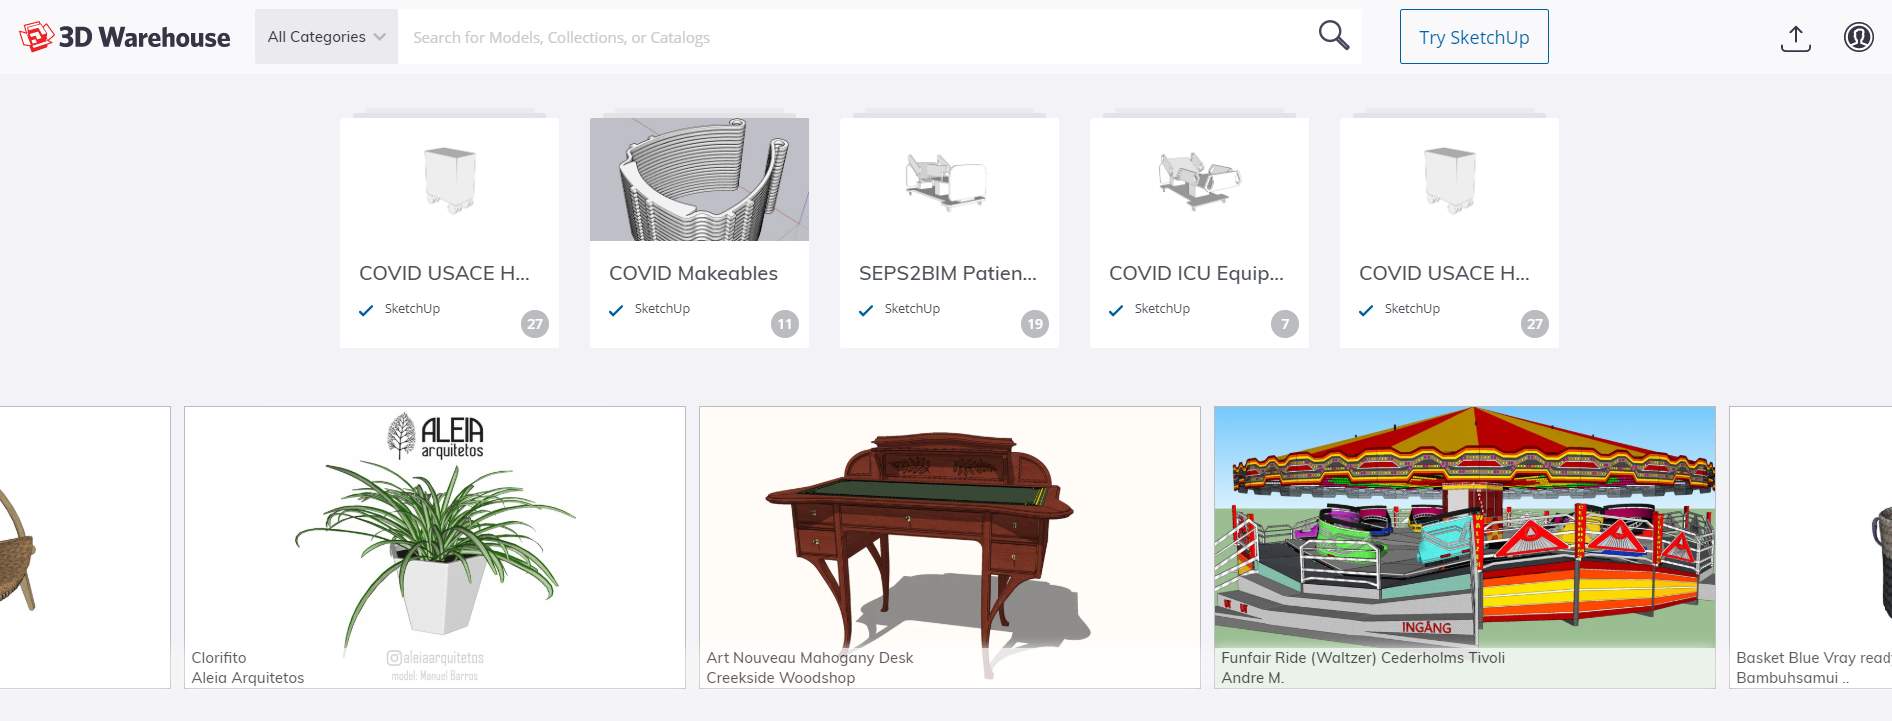
\includegraphics[width=450pt]{figuras/3dwh.png}
			\caption{3dwarehouse website}
			\label{3dwh}
		\end{figure*}
		
		Once the scenario has been choosed, the user should download the file as a COLLADA file as shown in \ref{ny} and then save the files at the \textit{meshes} directory explicited in \ref{cenario1}.
		
		
		\begin{figure*}[!ht]
			\centering
			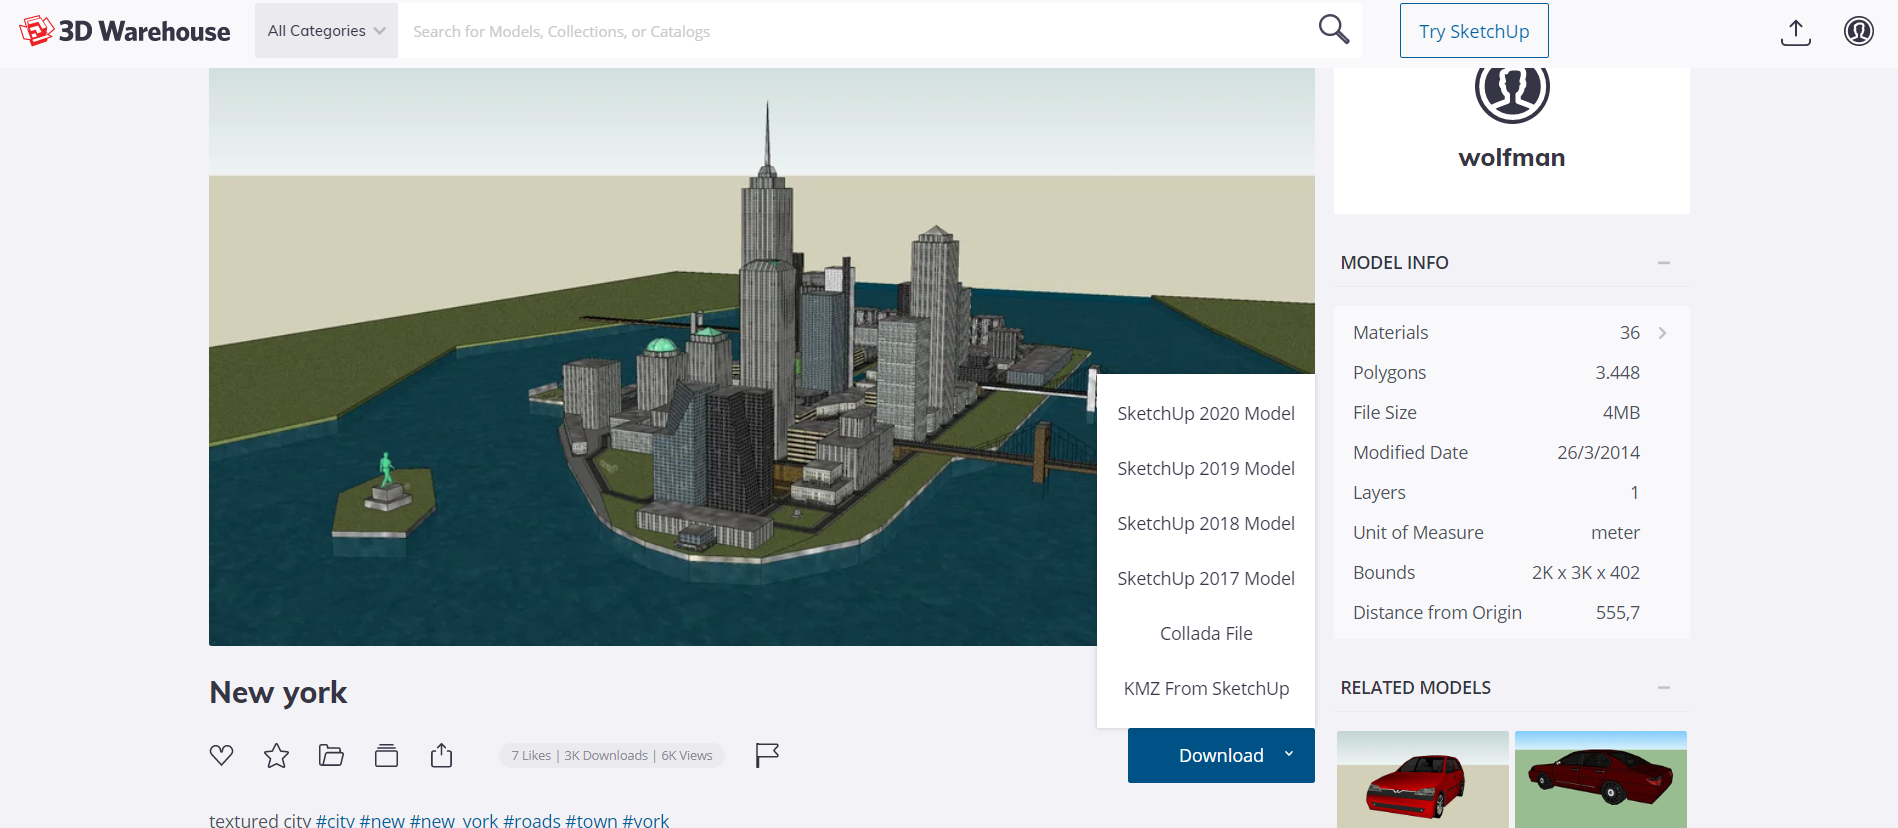
\includegraphics[width=350pt]{figuras/ny.png}
			\caption{Cenário}
			\label{ny}
		\end{figure*}
		
		
		\begin{figure*}[!ht]
			\centering
			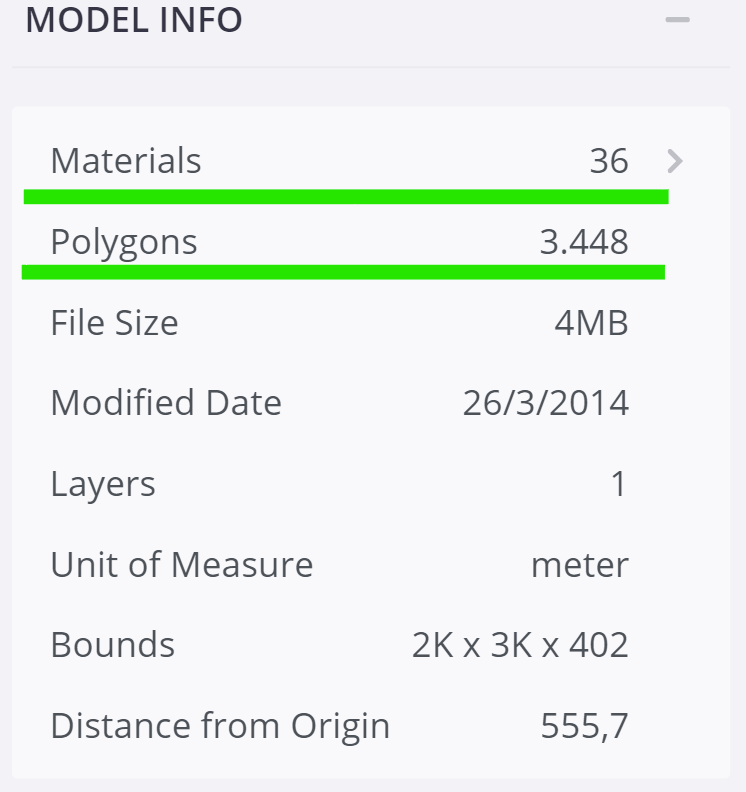
\includegraphics[width=150pt]{figuras/modelinfo.png}
			\caption{Numero de \textit{Polygons}}
			\label{modelinfo}
		\end{figure*}
		
		Some information have to be analysed from the 3dwarehouse website. In the \textit{model info} section of figure \ref{modelinfo} is possible to note the \textit{Polygon} parameter. A polygonal mesh is a collection of vertices, edges and faces that define the form of a 3D object. A high count of \textit{Polygons} demands vastly from the GPU and can slow down the simulation. 
		
		In order to avoid such problem the user must choose a scenario with a low \textit{Polygon} count or use a \textit{mesh modifier} to reduce the \textit{Polygon} count. The second option shall be treated in the next section.

		
		
		\section{Treating the Scenario}
		
		To decrease the number of \textit{Polygon} count the use of a \textit{mesh modifier} is necessary, in this case, Blender's \textit{Decimate Modiifer} is the \textit{mesh modifier} chosen. The first step is to download Blender.
		Once Blender is installed, the ".dae" file from the \textit{meshes} directory should be imported. Then, in the right corner menu the user should select the mesh modifier.
			
			\begin{figure*}[!ht]
			\centering
			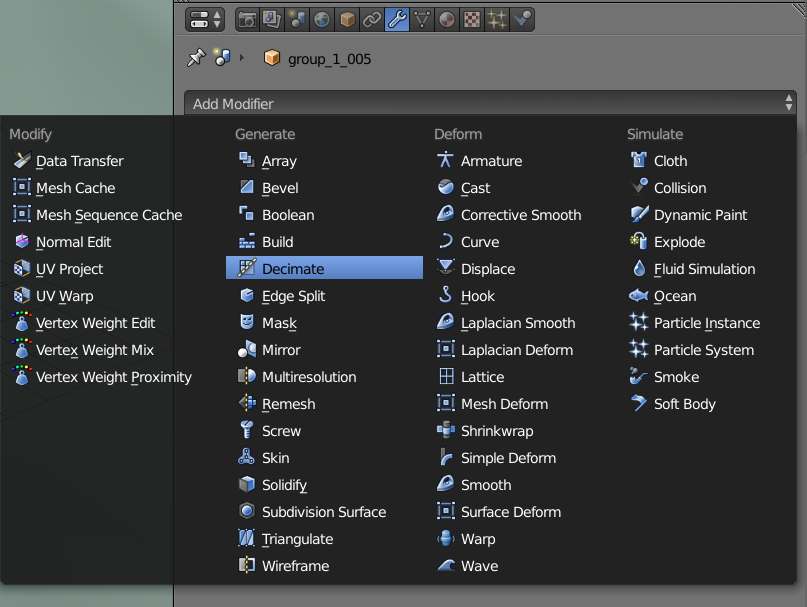
\includegraphics[width=250pt]{figuras/decimod.png}
			\caption{\textit{Decimate Modifier}}
			\label{decimod}
			\end{figure*}
		
		There are three available options for simplifying the mesh: \textit{Collapse},\textit{Un-subdivide} and \textit{Planar}.
		\begin{itemize}
			\item \textbf{\textit{Collapse}}:
			
			Progressively unites the vertices taking in to account the mesh shape. There are four parameters in this modifier:
			\begin{itemize}
				\item [-] \textit{Ratio}: Define the collapsed vertices ratio. If the values is equal to 1, the mesh is not altered, if the value is 0.5 half of the faces are collapsed, and if the values equals to 0 all faces have been removed.
				\item [-] \textit{Factor}: The amount of influence the Vertex Group has on the decimation.
				\item [-] \textit{Triangulate}: Keeps any resulting triangulated geometry from the decimation process.
				\item [-] \textit{Symmetry}: Maintains symmetry on a single axis.
			\end{itemize}
		\begin{figure*}[!ht]
			\centering
			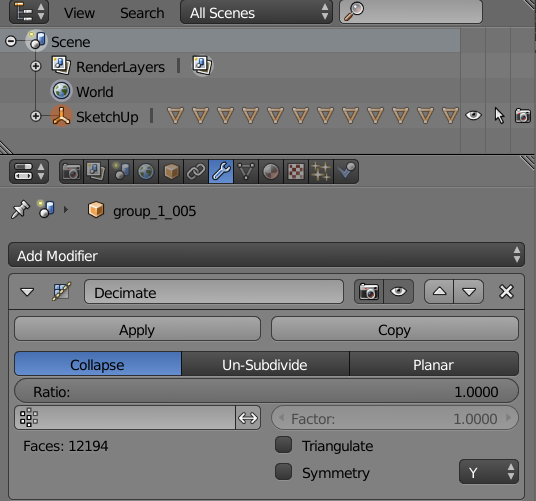
\includegraphics[width=200pt]{figuras/hillblendermod.png}
			\caption{\textit{\textit{Collapse}}}
			\label{collapse}
		\end{figure*}
		\item \textbf{\textit{Un-subdivide}}:It can be thought of as the reverse of subdivide. It attempts to remove edges that were the result of a subdivide operation. It is intended for meshes with a mainly grid-based topology (without giving uneven geometry). If additional editing has been done after the subdivide operation, the results may be unexpected.
		\begin{itemize}
			\item [-] \textit{Iterations}:The number of times to perform the un-subdivide operation. Two iterations is the same as one subdivide operation, so you will usually want to use even numbers.
		\end{itemize}
	\begin{figure*}[!ht]
		\centering
		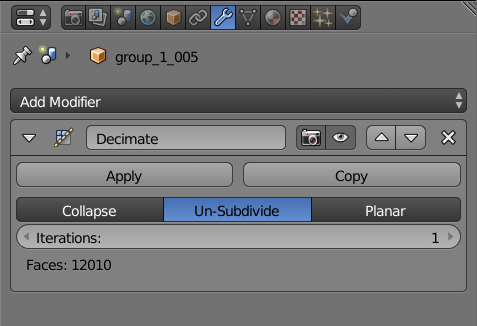
\includegraphics[width=200pt]{figuras/unsubdiv.png}
		\caption{\textit{\textit{Un-subdivide}}}
		\label{unsubdiv}
	\end{figure*}
		\item \textbf{\textit{Planar}}:It reduces details on forms comprised of mainly flat surfaces.
		\begin{itemize}
			\item [-] \textit{Angle Limit}:Dissolve geometry which form angles (between surfaces) higher than this setting.
			\item [-] \textit{All Boundaries}: When enabled, all vertices along the boundaries of faces are dissolved. This can give nicer results when using a high Angle Limit.
			\item [-] \textit{Delimit}: Prevent dissolving geometry in certain places.
		\end{itemize}
		\begin{figure*}[!ht]
		\centering
		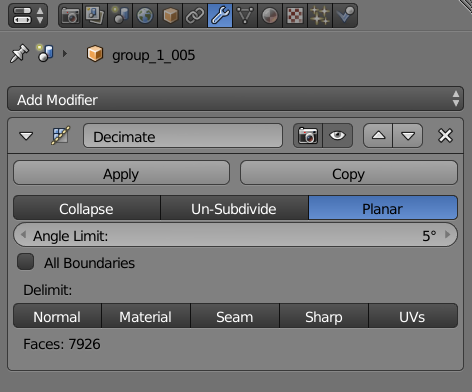
\includegraphics[width=200pt]{figuras/planar.png}
		\caption{\textit{\textit{Planar}}}
		\label{planar}
		\end{figure*}
		\end{itemize}
		
		At the top left menu the user should export the modified file with the ".dae" extension to the \textit{meshes} directory following the organization showned in \ref{cenario1}.

		
		
		\section{Scenario Configuration}
		
		Once the ".dae" file is treated is then necessary to start to configure the directories and files as showned in \ref{cenario1}

			\begin{bashcode}
			$HOME/catkin_ws/src/ProVANT-Simulator/source/Database/models/
			\end{bashcode}
		
	The user should configure the "model.sdf" file as visual link only as showned bellow.			

			
			\begin{minted}{xml}
	<model name="scenario_name">
		<pose>0 0 0  0 0 0</pose>
			<static>true</static>
				<link name="link_name">
				<visual name="scenario_visual_name">
				 <pose>0 0 0 0 0 0</pose>
				  <geometry>
					<mesh>
			<uri>model://scenario_directory_name/meshes/dae_file_name.dae</uri>
					</mesh>
				  </geometry>
				</visual>
			   </link>
			</model>
		</sdf>
		\end{minted}
		\centerline{Code: "model.sdf" description for a scenario}	
			
	    In the "meshes" directory the ".dae" files modified in blender as well as any texture file should be included. The "config.xml" file must be the same file from the uav the user intends to use with the scenario during the simulation.
		
		\begin{minted}{xml}
	
		<config>
	    <topicdata>data</topicdata>
		<TopicoStep>Step</TopicoStep>
		<Sampletime>12</Sampletime>
		<Strategy>Control_Strategy_of_Desired_UAV</Strategy>
		<RefPath>ref.txt</RefPath>
		<Outputfile>out.txt</Outputfile>
		<InputPath>in.txt</InputPath>
		<ErroPath>erro.txt</ErroPath>
		<Sensors>
			<Device>Topic_to_Receive_States_of_Desired_UAV</Device>
		</Sensors>
		<Actuators>
			<Device>Actuator_of_Desired_UAV</Device>
			.
			.
			.
			<Device>Actuator_of_Desired_UAV</Device>
		</Actuators>
		</config>
				\end{minted}
			\centerline{Code: "config.xml" description for a scenario}	
		
	\begin{itemize}
	\setlength{\itemsep}{1pt}
	\setlength{\parskip}{0pt}
	\setlength{\parsep}{0pt}
	\item[-] \textcolor{blue}{<Strategy></Strategy>}: especify the control strategy binary of the chosen uav;
	\item[-] \textcolor{blue}{<Sensors></Sensors>}: topic where the uav states are published;
	\item[-] \textcolor{blue}{<Actuators></Actuators>}: topics that receive the control signals and apply to the uav;
	\end{itemize} \normalsize
	
	The "model.config" file can be configures as showned:
	
	\begin{minted}{xml}
	<model>
		<name>scenario_name</name>
		<version>1.0</version>
		<sdf version="1.4">robot/model.sdf</sdf>
		<author>
			<name></name>
			<email></email>
		</author>
		<description></description>
	</model>
	\end{minted}
	\centerline{Code: "model.config" file description for a scenario}
	
	
		\begin{bashcode}
	$HOME/catkin_ws/src/ProVANT-Simulator/source/Database/worlds/worlds
\end{bashcode}
	The ".world" file must be configured as follows:	
	\begin{minted}{xml}
<world name="/HOME/catkin_ws/src/ProVANT-Simulator/source/Database/worlds/worlds
/scenario_world_directory/file_name.world">
	<gravity>0 0 -9.8</gravity>
	<physics type="ode">
		<max_step_size>0.001</max_step_size>
		<real_time_factor>0</real_time_factor>
	</physics>
	<plugin name="gazebo_tutorials" filename="libgazebo_ros_world_plugin.so">
		<ok>nothil</ok>
	</plugin>
	<include>
		<uri>model://sun</uri>
		<static>true</static>
	</include>
	<include>
		<uri>model://Desired_UAV</uri>
		<name>Arbitrary_name_to_appear_in_Gazebo</name>
		<static>false</static>
		<pose>0 0 0 0 0 0</pose>
	</include>
	<include>
		<uri>model://Desired_scenario_from_models_directory</uri>
		<name>Arbitrary_name_to_appear_in_Gazebo</name>
		<static>true</static>
		<pose>0 0 0 0 0 0</pose>
	</include>
	<scene>
		<sky>
			<time>18</time>
			<clouds>
			<speed>0</speed>
			</clouds>
		</sky>
	</scene>
</world>
</sdf>
	\end{minted}
	\centerline{Code: ".world" file description for a scenario}	
	
	\section{Example}
		\subsection{UAV 4.0 Scenario}
		
	The first step is to download the file and using the option \textit{import} in the top menu \textit{File} tab on Blender open the ".dae" file as showned in \ref{hillblender} 	
		

	\begin{figure*}[!ht]
	\centering
	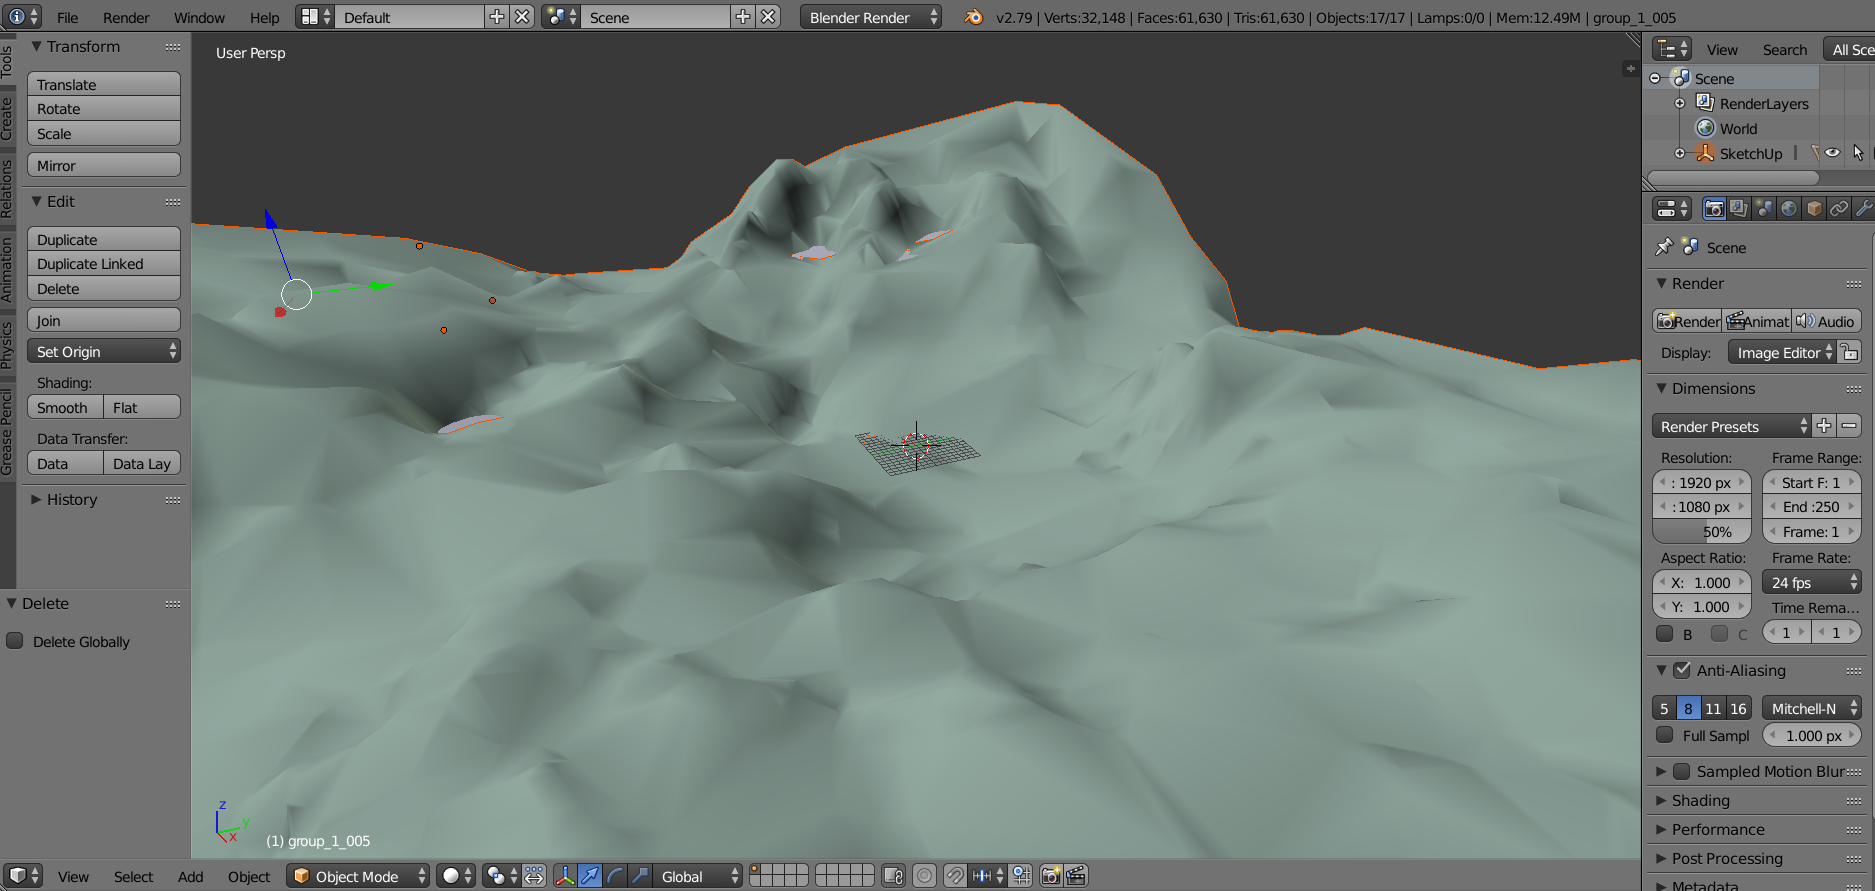
\includegraphics[width=350pt]{figuras/hillblender.png}
	\caption{Scenario in Blender}
	\label{hillblender}
\end{figure*}

	
	In the right menu of blender the user should select one of the three options presented in the \textit{modifiers} tab: \textit{Collapse}, \textit{Un-subdivide} or \textit{Planar}. In the application the option \textit{Collapse} was chosen so the vertices woulb progressively joined but keeping the mesh shape into account. In this case the parameter to b modified is the \textit{ratio} parameter, which defines the collapsed vertices ratio. As presentd in the sections above, a ratio value of 1 keeps the mesh unchanged. It's possible to follow the number of removed faces when using a \textit{modifier} by checking the \textit{faces} option shown in \ref{hillblendermod}. It's important that after the \textit{modifiers} are applied the user must select the \textit{Apply} option so the changes are saved.
	
	
		\begin{figure*}[!ht]
		\centering
		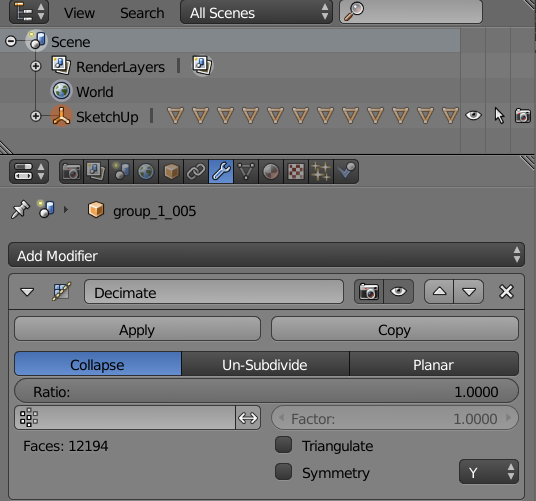
\includegraphics[width=250pt]{figuras/hillblendermod.png}
		\caption{\textit{Collapse} in 3D Blender}
		\label{hillblendermod}
	\end{figure*}
	
	Once the modifications are saved the user should export the model as a ".dae" file using the top left menu \textit{File} tab and selecting the \textit{export} option. Create the directories and files as showned in \ref{cenario1} and then save the ".dae" file in the \textit{meshes} directory of the scenario model. In this case, the file is on the path bellow:

	
	\begin{bashcode}
	$HOME/catkin_ws/srcProVANT-Simulator/source/Database/models/cenario_hill/meshes	
		\end{bashcode}
	\label{daefile}
	

At the \textit{meshes} directory, besides of the ".dae" file, the textures files should also be included as shown in \ref{mesheshill}



			\begin{figure*}[!ht]
	\centering
	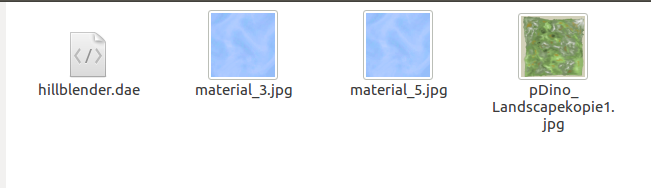
\includegraphics[width=350pt]{figuras/mesheshill.png}
	\caption{\textit{meshes} Directory}
	\label{mesheshill}
\end{figure*}

The scenario "model.sdf" file must be configured then. To do so the user should head to the scenario model diretory and at the "robot" directory open the "model.sdf" file with the user's editor of preference.  
				\begin{bashcode}
	$HOME/catkin_ws/src/ProVANT-Simulator/source/Database/models/cenario_hill/robot	
\end{bashcode}

			\begin{figure*}[!ht]
	\centering
	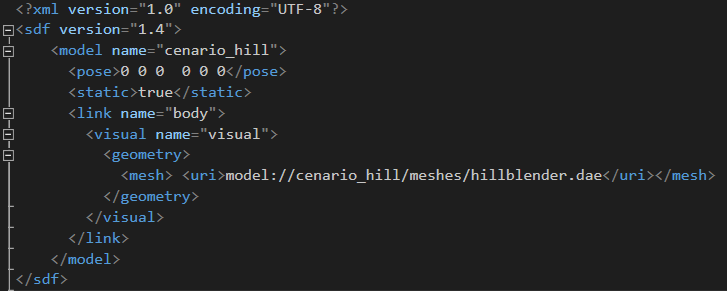
\includegraphics[width=350pt]{figuras/excenario.png}
	\caption{Scenario "model.sdf" file example}
	\label{excenario}
	\end{figure*}

The scenario "model.sdf" file should only contain a link with visual properties as showned in \ref{excenario}. The "model.config" file must be configured as \ref{ex2cenario} with the appropriate description.



			\begin{figure*}[!ht]
	\centering
	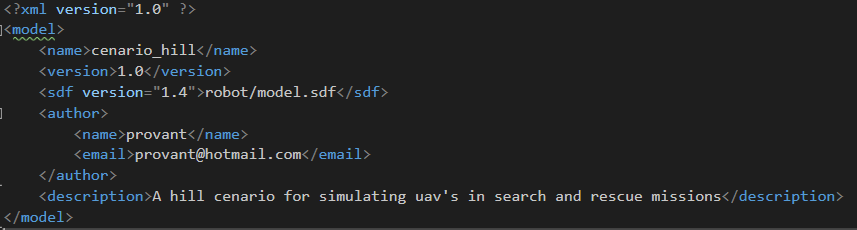
\includegraphics[width=350pt]{figuras/ex2cenario.png}
	\caption{Scenario "model.config" file example}
	\label{ex2cenario}
\end{figure*}

Still at the scenario model directory the user should configure the 'config.xml" file. Definig UAV 4.0 (\ref{vant4}) as the simulation uav, both uav "config.xml" file and the scenario "config.xml" file should be the same. This is due the internal simulator software organization. The file is configured as shown in \ref{ex3cenario}.

			\begin{figure*}[!ht]
	\centering
	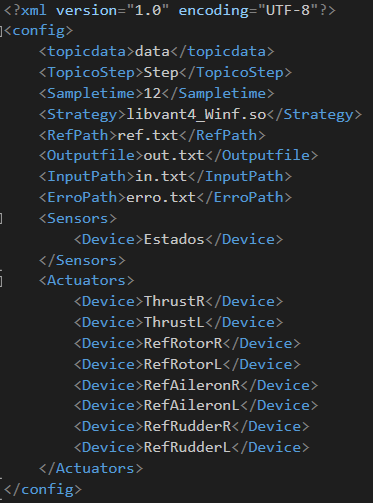
\includegraphics[width=200pt]{figuras/ex3cenario.png}
	\caption{Scenario "config.xml" example when using UAV 4.0.}
	\label{ex3cenario}
\end{figure*}

Then the user should create the directories and files as in \ref{cenario2}. In this example, the directory where the ".world" file is located is the Hill directory at the \ref{worldshill} path.


				\begin{bashcode}
	$HOME/catkin_ws/src/ProVANT-Simulator/source/Database/worlds/worlds/Hill	
	\end{bashcode}
\label{worldshill}

The ".world" file is configured as showned in figure \ref{ex4cenario}

			\begin{figure*}[!ht]
	\centering
	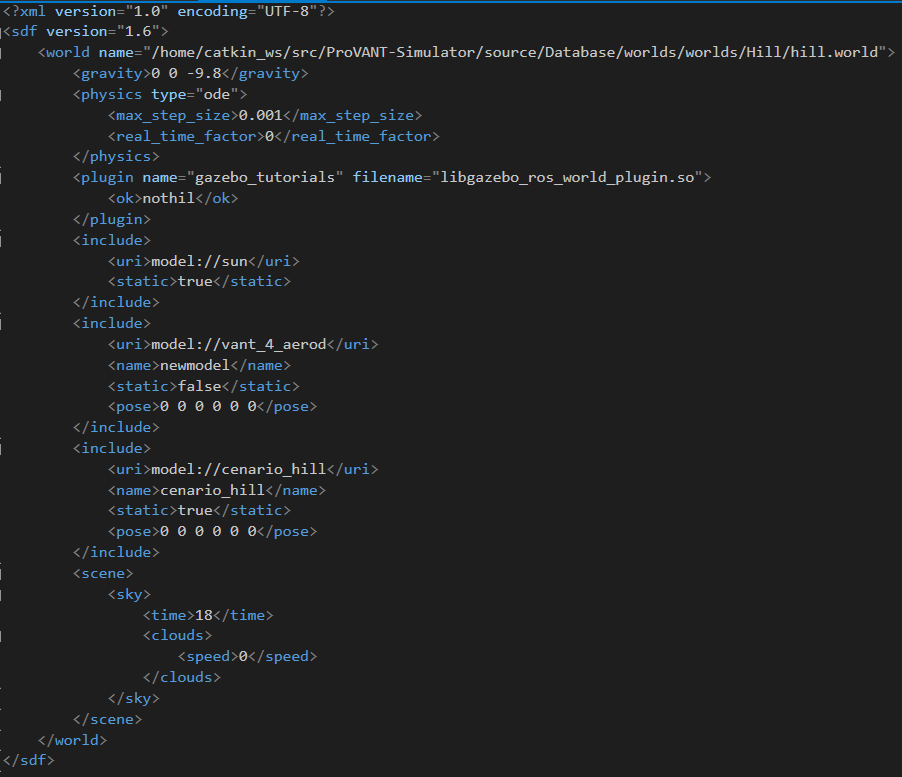
\includegraphics[width=350pt]{figuras/ex4cenario.png}
	\caption{".world" File configured for a scenario using UAV 4.0.}
	\label{ex4cenario}
\end{figure*}

It's important to understand the \textit{tags} that include both the UAV and the scenario model.
\begin{minted}{xml}
<include>
	<uri>model://vant_4_aerod</uri>
	<name>newmodel</name>
	<static>false</static>
	<pose>0 0 0 0 0 0</pose>
</include>
<include>
	<uri>model://cenario_hill</uri>
	<name>cenario_hill</name>
	<static>true</static>
	<pose>0 0 0 0 0 0</pose>
</include>
 \end{minted}
	\centerline{Code: Including UAV and scenario model in the ".world" file.}


\begin{itemize}
	\itemsep0em
	\item[-] <uri></uri>: Search for the UAV and scenario models in the \textit{model} directory.
	\item[-] <name></name>: UAV and Scenario names displayed in Gazebo.
	\item[-] <static></static>: Indicates if the object is static in the simulation.
	\item[-] <pose></pose>: For the uav, the pose should be the same as the pose for the uav without scenario, and for the scenario the pose should be the one displayed in the figured. 
\end{itemize}

Doing so the simulation will be ready to be launched. To start the UAV 4.0 with scenario simulation the user should follow the steps presented in section \ref{workflow} examples.

			\begin{figure*}[!ht]
	\centering
	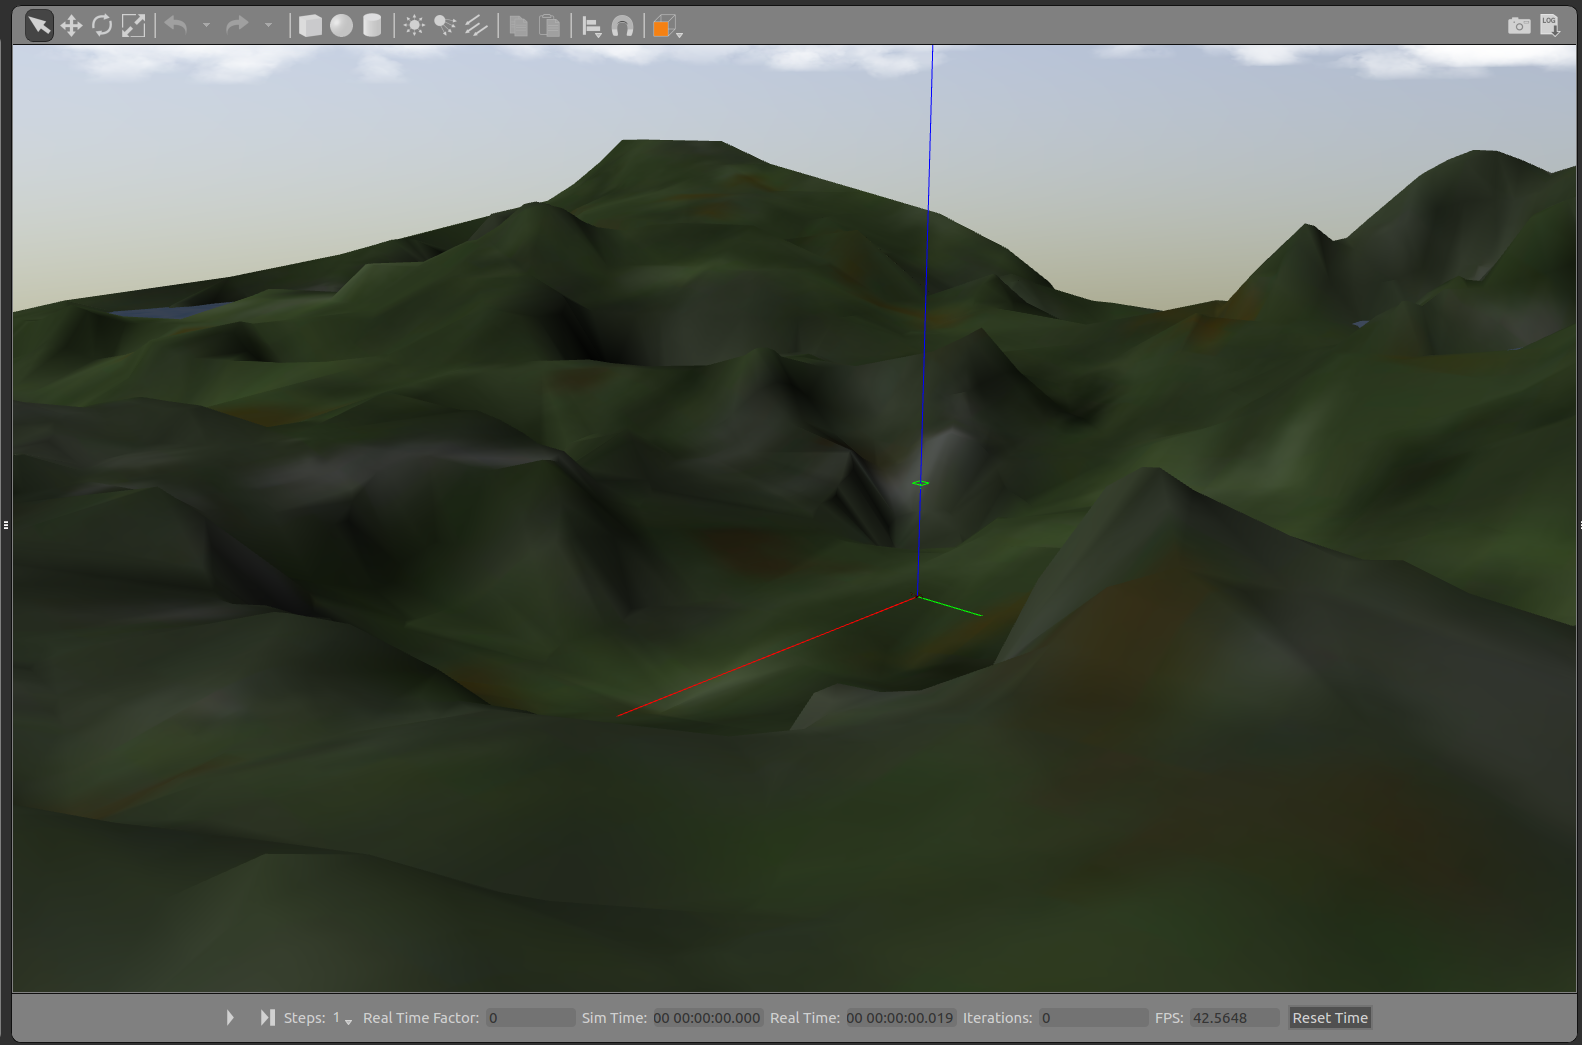
\includegraphics[width=350pt]{figuras/exhill.png}
	\caption{UAV 4.0 with Scenario Simulation}
	\label{exhill}
\end{figure*}